\section{Durchführung und Aufbau}
\label{sec:Durchführung}
Ziel des Versuches ist es sich mit den Grundlagen der Vakuumtechnik vertraut zu machen und das Saugvermögen von einer Drehschieberpumpe als auch einer Turbopumpe zu bestimmen. Eine Skizze des Aufbaus ist in Abbildung \ref{fig:pump} zu sehen.
\begin{figure}[htpb]
  \centering
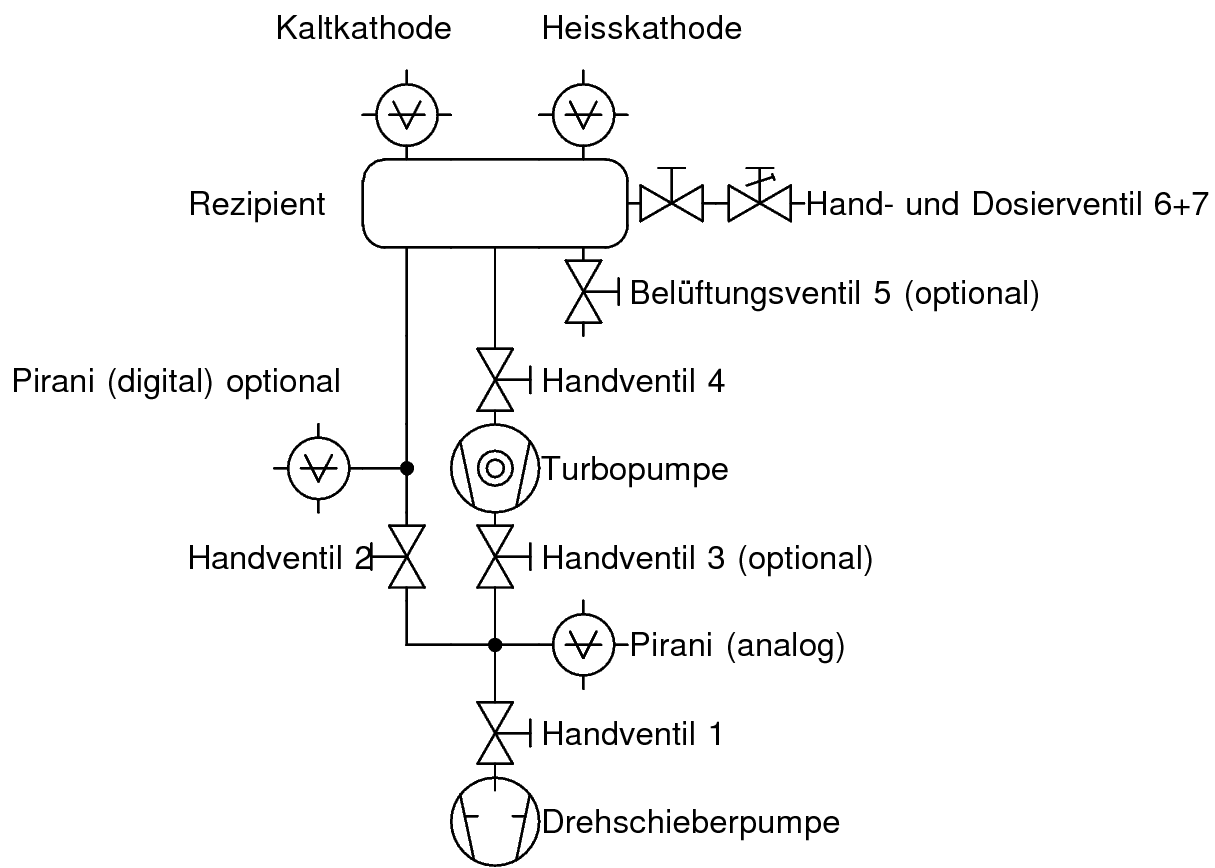
\includegraphics[width=0.8\textwidth]{picture/pumpaufbau.png}
\caption{Schema des Aufbaus des Pumpstandes \cite{Pfeiffer}}
  \label{fig:pump}
\end{figure}
Beim Aufbau des Vakuumstandes wurde darauf geachtet, einen Pumpstand mit einem geringen Volumen zu konzipieren um diesen möglichst übersichtlich zu halten. Alle Dichtungen sind handfest zugezogen und der Rezipient erwärmt worden, um das Ausgasen zu verringern. Desweiteren wird um die Auswirkung von virtuellen Lecks zu minimieren der Rezipient mit einem Föhn erwärmt. Dadurch erhöht sich zunächst die Desorptionsrate, jedoch nimmt diese mit Abkühlen des Rezipientns wieder ab und im Anschluss sind kleinere Enddrücke $p_\text{E}$ zu errreichen.
\subsection{Messbereiche}
Aufgrund eines Defekts des Kaltkathodenmessgeräts standen nur das Pirani- sowie, dass Heißkathoden-Messgerät zur Verfügung. Zur Bestimmung der Messgrößen der Drehschieberpumpe wurde deshalb ausschließlich das Piranimessgerät benutzt, weil die Glühkathode des Heißkathodenmessgeräts im hohen Druckbereich durchbrennen würde. \newline
Zur Bestimmung der Messgrößen der Turbopumpe wird das Pirani-Messgerät hinter die Drehschieberpumpe geschaltet um zu prüfen ob das entsprechende Vorvakuum zur Inbetriebnahme der Turbopumpe erreicht wird. Hinter die Turbopumpe wird anschließend das Glühkathodenmessgerät geschaltet um den Druck im Rezipienten bei der Inbetriebnahme der Turbopumpe zu bestimmen.
\subsection{Messungen an der Drehschiebepumpe}
Zur Bestimmung der Messgrößen der Drehschieberpumpe wird der Versuch wie in Abbildung \ref{fig:Dreh} abgebildet aufgebaut.
\begin{figure}[htpb]
  \centering
  \includegraphics[width=\textwidth]{picture/Aufbau1.png}
  \caption{Pumpstand zur Bestimmung des Saugvermögens der Drehschieberpumpe}
  \label{fig:Dreh}
\end{figure}
Der Rezipient (1) wird mittels einer Verbindung (2) anhand eines T-Stückes (5) an ein Ablassventil (3) gekoppelt welches mittels eines Ventils (4) vom Versuch abgeklemmt werden kann. Anschließend folgen zwei T-Stücke (6 \& 8) welche keine gesonderte Funktion haben außer die Kammer um eine Ecke zu lenken. Anschließend folgt ein T-Stück an welchem das Pirani-Messgerät (7) geschaltet ist um den Druck im Rezipienten zu messen. Abschließend folgt ein Ventil (9) um den Rezipienten von der Drehschieberpumpe zu trennen um Leckratenmessungen durchführen zu können. \newline
Zunächst soll die $p(t)$-Kurve aufgenommen werden. Als erstes wird dafür der Enddruck $p_\text{e}$ der Drehschieberpumpe gemessen. Dazu muss das Überdruckventil geschlossen werden und der Druck durch die analoge Anzeige des Pirani-Messgerät abgelesen werden. Anschließend wird für vier verschiedene Drücke jeweils zu 18 verschiedenen Drücken die Zeit genommen welche die Pumpe benötigt um diese zu erreichen. Die Messreihe wird jeweils 5-mal durchgeführt. \newline
Anschließend wird die Leckrate bestimmt indem das Nadelventil (3) so justiert wird, dass sich zwischen Saugvermögen und Luftsstrom ein Gleichgewichtsdruck von (0.1, 0.4, 0.8 und 1.0) \cdot $10^{-2}$ mbar eingestellt. Anschließend wird die Pumpe abgeklemmt und der Druck gegen die Zeit aufgenommen. Dies wird für jeden Gleichgewichtsdruck 3 mal wiederholt.  \newline
\subsection{Turbomolekularpumpe}
Um für die Turbopumpe ein hinreichend großes Vorvakuum zu produzieren muss der Aufbau modifiziert werde. Dafür wird der Zugang zur Drehschieberpumpe vom T-Stück an die Turbopumpe ummontiert und das T-Ventil mit einem Flansch geschlossen. In Abbildung \ref{fig:Turbo} ist der Aufbau dargestellt.
\begin{figure}[htpb]
  \centering
  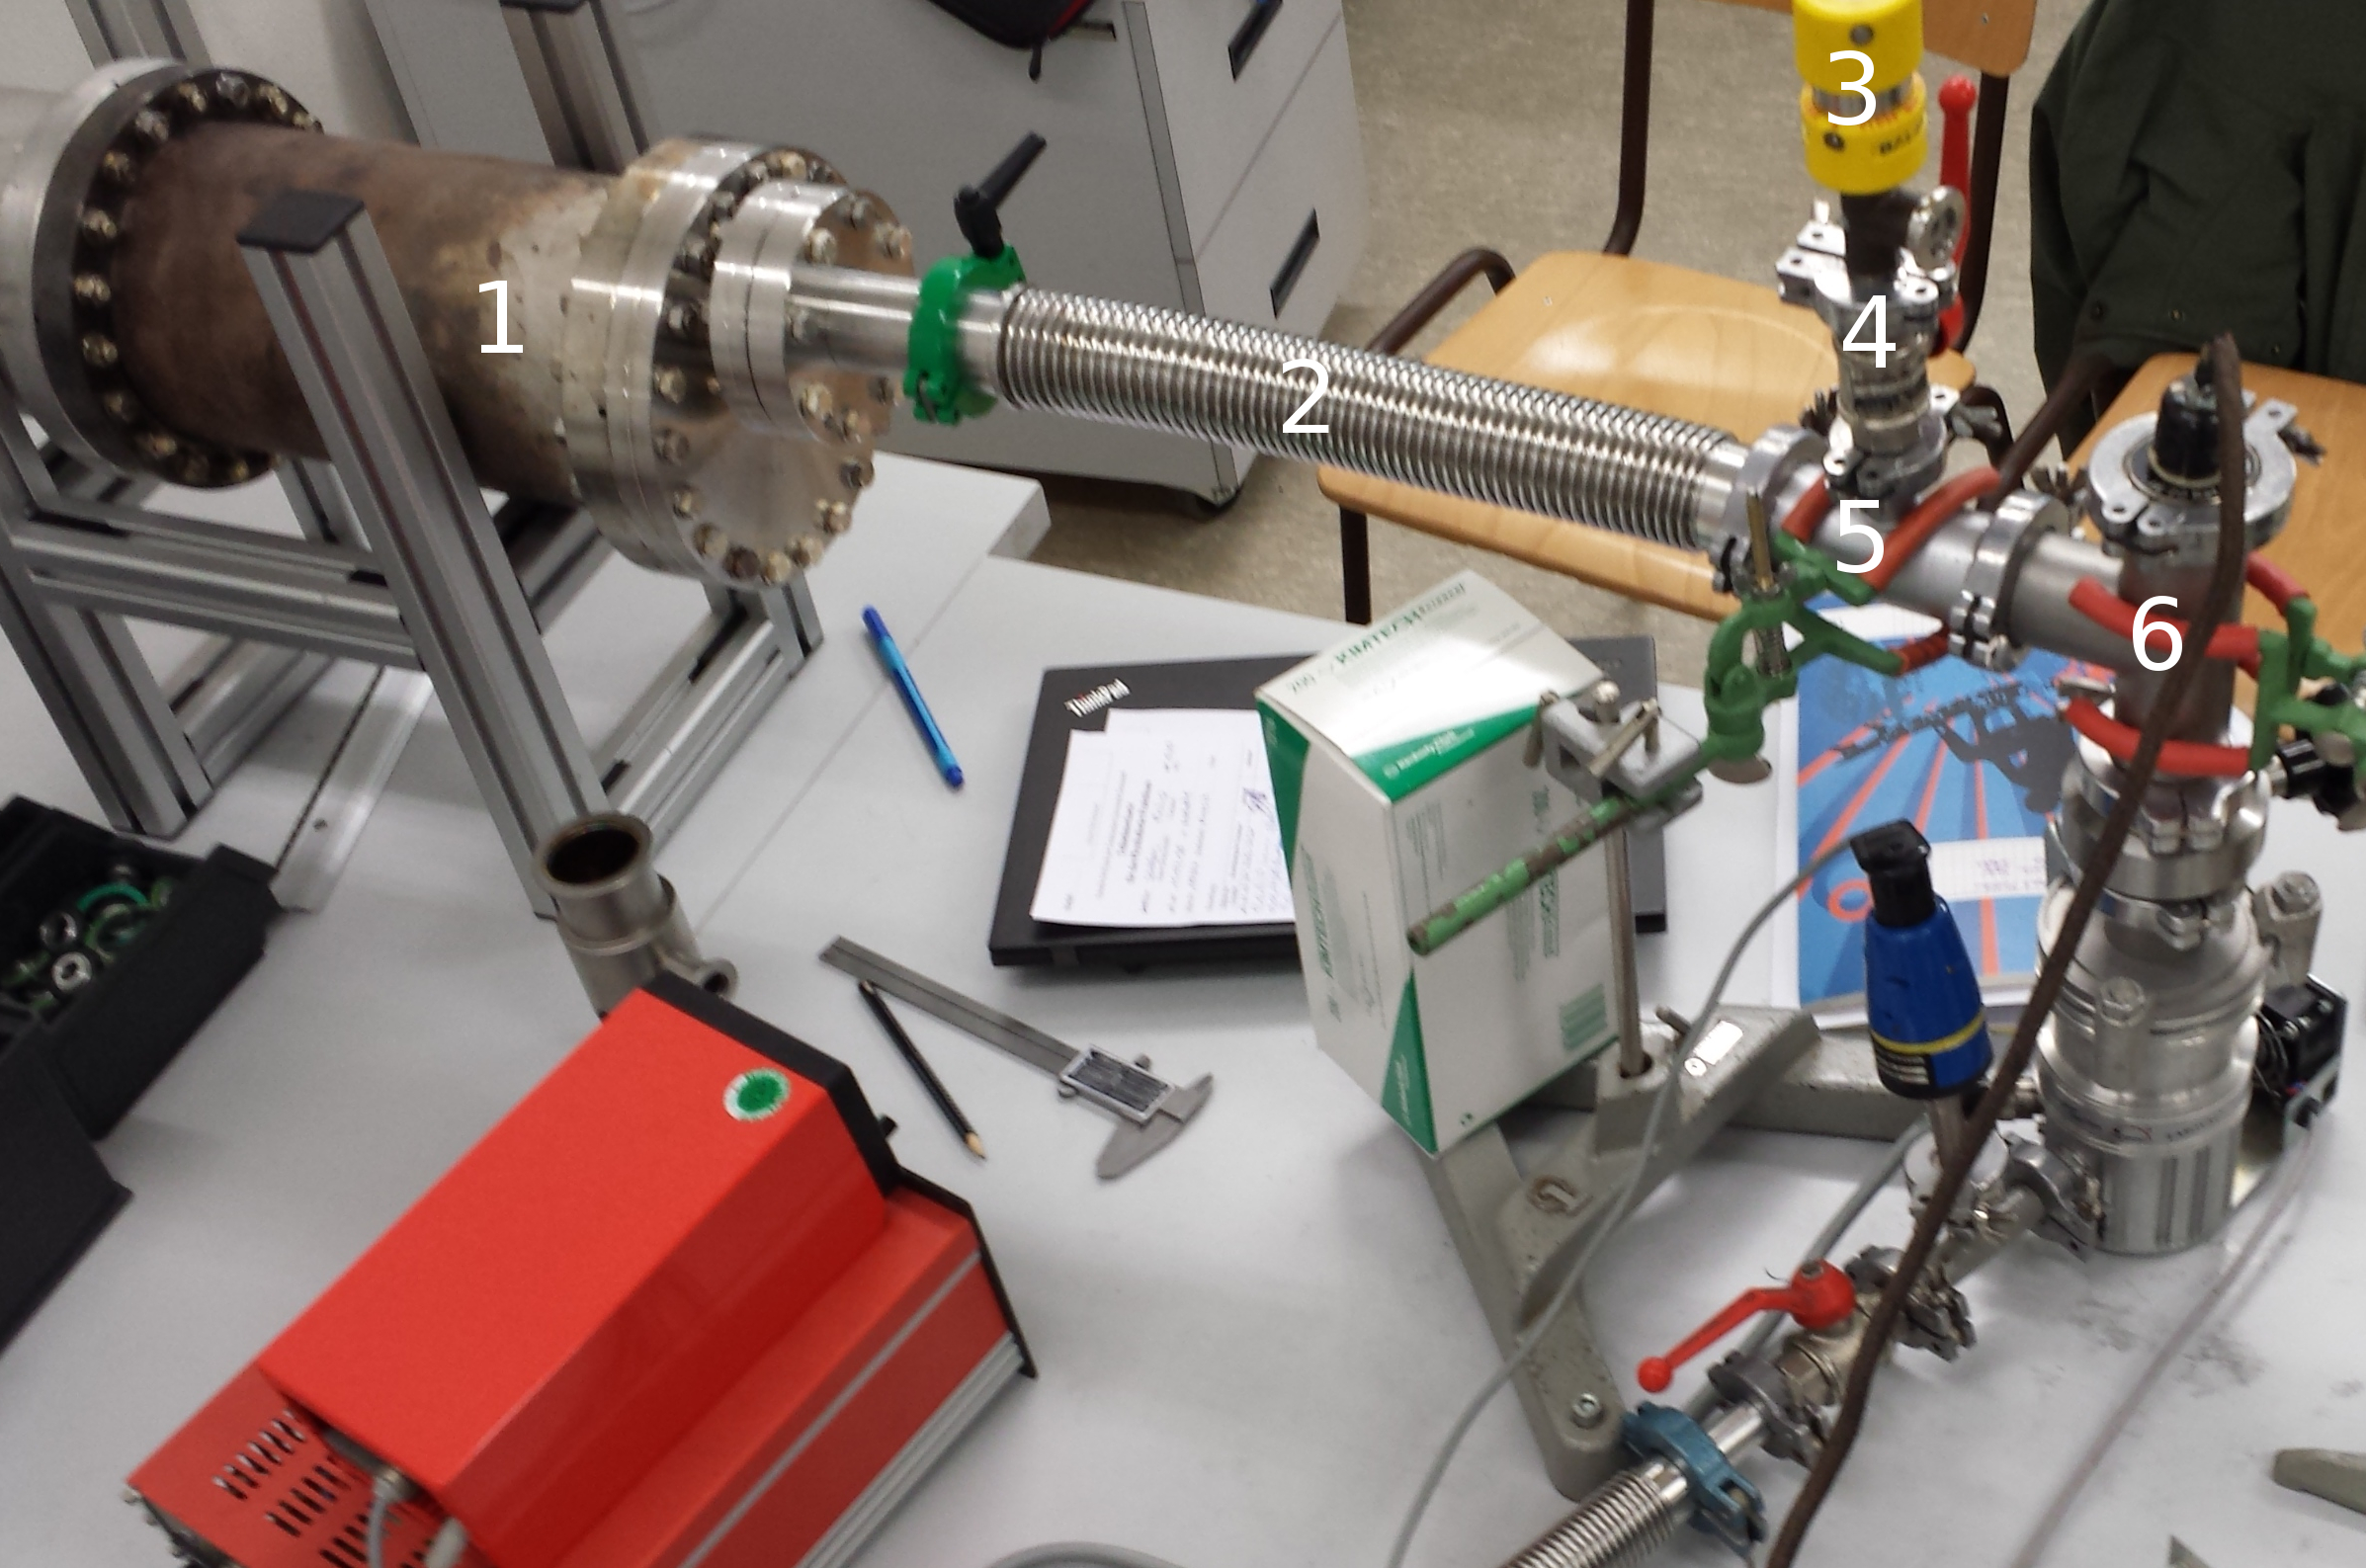
\includegraphics[width=\textwidth]{picture/Aufgabe2.jpg}
  \caption{Aufbau des Pumpstandes zur Messung des Saugvermögens der Turbomolekularpumpe}
  \label{fig:Turbo}
\end{figure}
Anschließend wird dieselbe Messreihe wie bei der Drehschiebepumpe aufgenommen, jedoch mit modifizierten Drücken. Es sollen 4 Leckratenmessreihen mit Startdrücken von 5 bis $20 \cdot 10^{-5}$ mbar durchgeführt werden und die $p(t)$-Messung jeweils von einem Druck von $5 \cdot 10^{-3}$ mbar jeweils 3 Messungen. Dabei tritt das Problem auf, dass die Glühkathode mit dem Ionenfänger verbunden ist und somit die Sicherung des Messgeräts vor dem Beheben des Problems immer wieder abschaltet. Desweiteren wird aufgrund der kurzen Zeitabstände der Druckverlauf gefilmt und am Computer mittels Movie-Maker ausgewertet, da eine exakte Zeitnahme per Hand schwer möglich schien.

\subsection{Volumenbestimmung der einzelnen Vakuumkomponenten}
Zuletzt werden die Maße der verwendeteten Rohre, Schläuche, Tank usw. genommen um das Volumen des evakuierten Raums zu berechnen. Aufgrund dessen, dass z.B. die Dicke der Tankewände nicht zu ermitteln ist, kann nur der Außendurchmesser bestimmt werden. Dementsprechend ist das Tankvolumen mit einer großen unsicherheit behaftet. 
\subsection{Nachbereitung}
Um virtuelle Lecks für die folgenden Gruppen zu minimieren wird der Rezipient und alle Pumpen nach Beendigung des Versuches mittels eines Blindflansch geschlossen.
